\section{Literature Review}

\begin{figure}[ht]
  \centering
  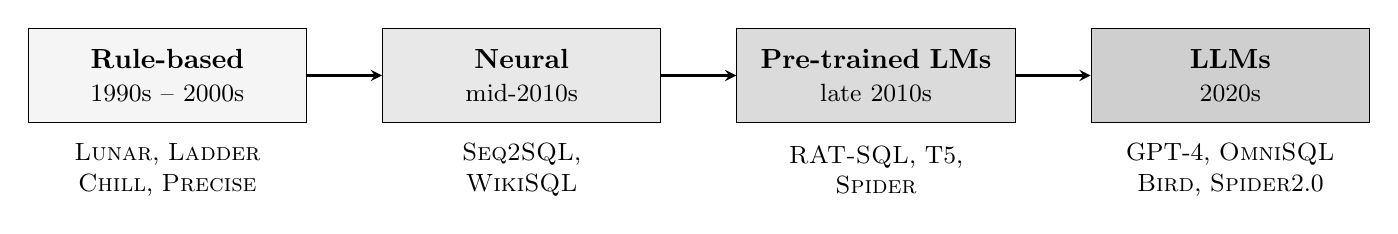
\begin{tikzpicture}[
    era/.style={draw, rectangle,
                minimum width=3.5cm, minimum height=1.2cm,
                text width=3.3cm, align=center},
    arr/.style={->, thick, >=stealth}
  ]
    \node[era, fill=gray!8]  (rule)   at (0,0)    {\textbf{Rule-based}\\{\small 1990s -- 2000s}};
    \node[era, fill=gray!18] (neural) at (4.5,0)  {\textbf{Neural}\\{\small mid-2010s}};
    \node[era, fill=gray!28] (plm)    at (9.0,0)  {\textbf{Pre-trained LMs}\\{\small late 2010s}};
    \node[era, fill=gray!38] (llm)    at (13.5,0) {\textbf{LLMs}\\{\small 2020s}};

    \draw[arr] (rule) -- (neural);
    \draw[arr] (neural) -- (plm);
    \draw[arr] (plm) -- (llm);

    \node[font=\small, align=center] at (0,-1.2)
      {\textsc{Lunar}, \textsc{Ladder}\\\textsc{Chill}, \textsc{Precise}};
    \node[font=\small, align=center] at (4.5,-1.2)
      {\textsc{Seq2SQL},\\\textsc{WikiSQL}};
    \node[font=\small, align=center] at (9.0,-1.2)
      {\textsc{RAT-SQL}, T5,\\\textsc{Spider}};
    \node[font=\small, align=center] at (13.5,-1.2)
      {GPT-4, \textsc{OmniSQL}\\\textsc{Bird}, \textsc{Spider}2.0};
  \end{tikzpicture}
  \caption{Paradigm shifts in NL2SQL research from rule-based systems to large language models, with representative systems and benchmarks.}
  \label{figure:nl2sql-paradigm-shifts}
\end{figure}

In this section a comprehensive literature review is performed to assess the research landscape on NL2SQL,
also referred to as Text-to-SQL or T2SQL and NLIDBs. From the time their development accelerated in
the late 1990s and early 2000s \citep{NLIDBs, NLIDBTheory, ILPParsing, ILPParsing2} until now, observing multiple
larger paradigm shifts happening over time \citep{GRAPPA, STRUG, Seq2SQL, NALIR, SQLizer}. In particular this
thesis focuses on the recent advancements when it comes to LLMs and how they
can be harnessed for effective NL2SQL systems \citep{LLM-Sql, DAIL-SQL,
T2SQL-LLM-Bench-2, T2SQL-LLM-Bench-3, Spider2, BIRD}.

This literature review covers the foundational concepts, challenges, key advancements and research gaps
associated with NL2SQL, establishing the context for this thesis and it's research questions.

\subimport{}{foundations}
\subimport{}{traditional-approaches}
\subimport{}{neural-approaches}
\subimport{}{pretrained-models}
\subimport{}{llm-approaches}
\subimport{}{benchmarking}
\subimport{}{research-gaps}
